% 2011 年湖南卷理科第 21 题：椭圆 C1 与抛物线 C2。
% 来源 PDF：普通高考/2011/2011湖南理.pdf，SHA-256 09b67f1db8e6a280165cf8431211a968163c0d0f262a50068dd607607a9ec578。
% 原页：第 2 页第 2 栏下部，书页码 672。示意。
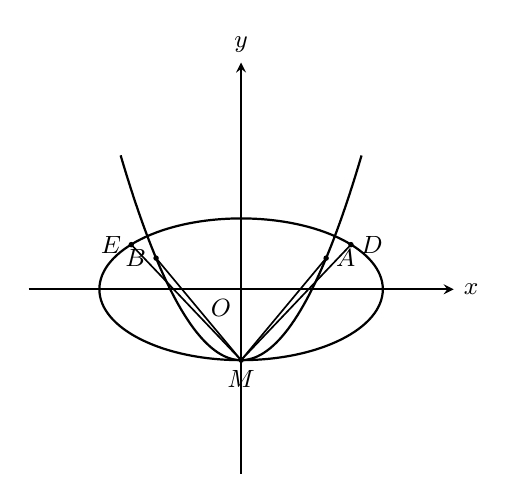
\begin{tikzpicture}[>=stealth, semithick, font=\small, scale=0.9]
  \draw[->] (-3,0)--(3,0) node[right] {$x$};
  \draw[->] (0,-2.6)--(0,3.2) node[above] {$y$};
  \draw[thick] (0,0) ellipse (2 and 1);
  \draw[thick, domain=-1.7:1.7, samples=80] plot (\x,{\x*\x-1});
  \coordinate (M) at (0,-1);
  \coordinate (A) at (1.2,0.44);
  \coordinate (B) at (-1.2,0.44);
  \coordinate (D) at (1.55,0.63);
  \coordinate (E) at (-1.55,0.63);
  \draw (A)--(M)--(B);
  \draw (D)--(M)--(E);
  \fill (M) circle (1.1pt) node[below] {$M$};
  \fill (A) circle (1.1pt) node[right] {$A$};
  \fill (B) circle (1.1pt) node[left] {$B$};
  \fill (D) circle (1.1pt) node[right] {$D$};
  \fill (E) circle (1.1pt) node[left] {$E$};
  \node[below left] at (0,0) {$O$};
\end{tikzpicture}
